Lowering the input resolution is the cheapest model-level saving
available. It needs no training, only a new engine. \Cref{fig:resolution}
compares static 512, 576 and 640 engines of the same pretrained YOLO26n
checkpoint on all of val2017, in the naive pipeline (float input,
sequential, stream sync) and in the full pipeline. Accuracy falls from
0.4026 AP (640) to 0.3864 (576) and 0.3748 (512). AP$_S$ falls from 0.198
to 0.175 and 0.160. In the naive pipeline, 512 buys 27\% more throughput
(34.3 to 43.4 images/s) and 22\% less energy per image. In the full
pipeline the same saving shrinks to a few percent: 214.6, 222.2 and
218.7 images/s for 640, 576 and 512 ($+3.5$\% and $+1.9$\%; the
repeat ranges of the lower resolutions lie above the 640 range, so
the gain is small but consistent across the two repeats). The pipeline is now limited by the main thread
(\cref{sec:ladder}): at 1020\,MHz the engine's 4.2\,ms sits just below
the ${\approx}4.7$\,ms per-image period the host stages impose, so most
of the engine time saved by a smaller input is absorbed by the
unchanged per-image host work.

Part of that saturation is Python. Re-running the same comparison with
CPython's cyclic garbage collector disabled (\texttt{gc.disable()},
identical predictions) raises all three throughputs to 229.9, 244.0 and
252.1 images/s, and the resolution spread widens to $+6.1$\% (576) and
$+9.7$\% (512). Cyclic-GC pauses on the main thread absorb a further
share of the saved engine time; with them removed, a lower input
resolution still buys roughly a third of what it buys in the naive
pipeline, not a negligible amount. The host work that remains ---
the main thread's per-image period
(\cref{sec:ladder}) --- depends on the source image and the pipeline,
not on the network input. The energy benefit is robust either way:
73.7 to 58.0\,mJ per image (21\%) on a backlog with the default
collector, and 71.2 to 55.8\,mJ (22\%) with it disabled, because the
GPU finishes each inference sooner. The same 2.8 AP
points therefore buy a large throughput gain in a naive pipeline and a
much smaller one in an optimized pipeline --- $2$--$10$\% depending on
host-runtime hygiene. A compression or resolution decision evaluated in a naive
pipeline, or in \texttt{trtexec}, does not carry over to an optimized one.

\begin{figure}[t]
\centering
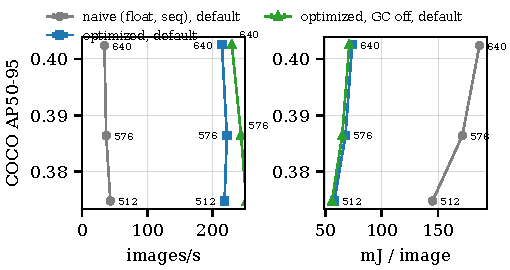
\includegraphics[width=\columnwidth]{figs/resolution.pdf}
\caption{COCO val2017 AP against throughput (images/s) and energy per
image (mJ) for
static 512/576/640 YOLO26n engines, default governors, mean of two runs
(whiskers: repeat min/max; labels: input size).
In the full pipeline (squares), lower resolution buys only $2$--$4$\%
throughput because the pipeline is limited by the main thread, not by
GPU throughput (the GPU already runs at its maximum clock); disabling
CPython's cyclic GC (triangles, identical predictions) raises all three
points and widens the spread to $6$--$10$\%.}
\label{fig:resolution}
\end{figure}
